\documentclass[12pt, a4paper]{article}  


\usepackage{amsmath,amsfonts,amssymb,amsthm,mathtools}  
\usepackage{graphicx}

\usepackage{fontspec}         
\setmainfont{Helvetica} 
\newfontfamily{\cyrillicfonttt}{Helvetica}
\newfontfamily{\cyrillicfont}{Helvetica}
\newfontfamily{\cyrillicfontsf}{Helvetica}   

\usepackage{unicode-math}     
   

\usepackage{polyglossia}      
\setdefaultlanguage{russian}  
\setotherlanguage{english}    
\begin{document} 
\section{Десять фактов обо мне}
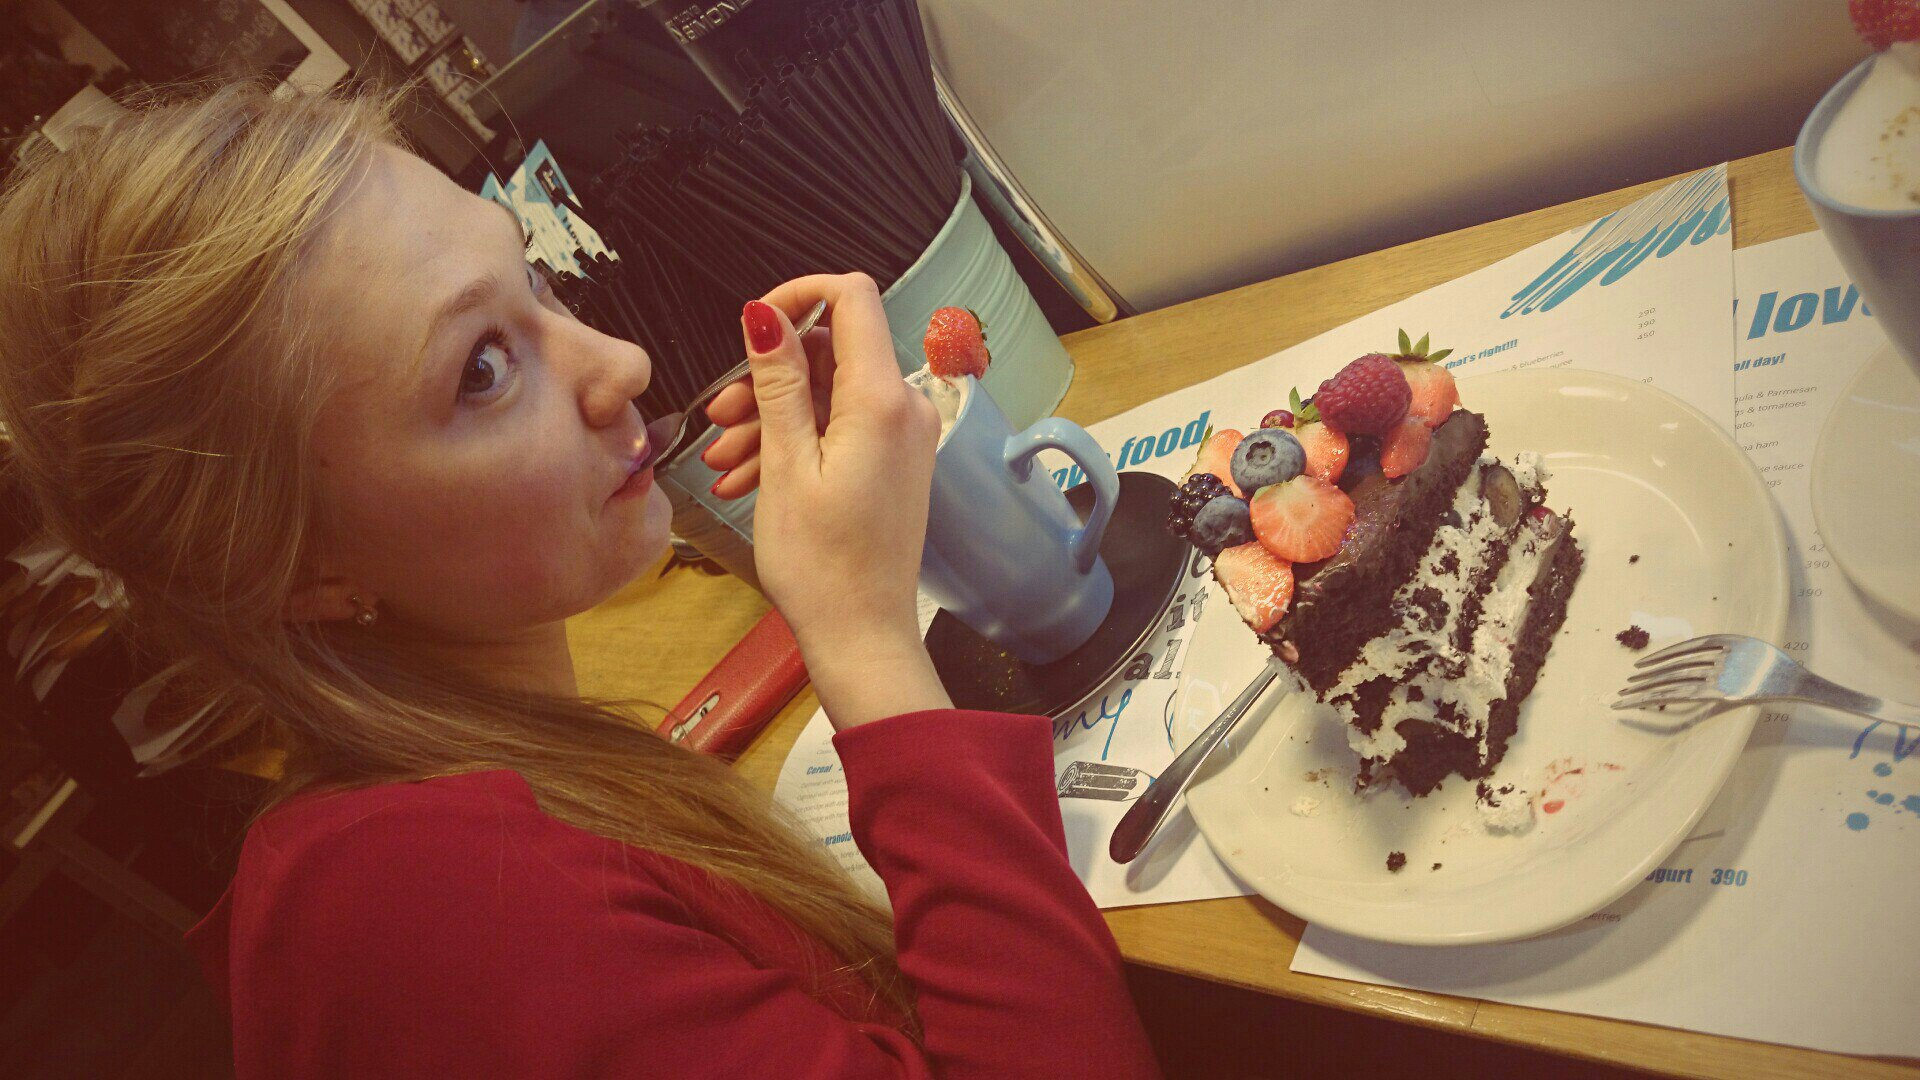
\includegraphics[scale=0.15]{ph1.png}
\begin{enumerate}
\item Никогда не смотрела фильмы ужасов
\item Боюсь кататься на качелях, а вот на всяких американских горках люблю
\item В детстве на шахматных турнирах "сливала" партии, потому что "захотела покушать"
\item Люблю старые фильмы
\item Часто при просмотре фильма смотрю сначала его конец
\item Летом я таю как Снегурочка и сгораю до состояния вареного краба, поэтому предпочитаю выходить только ночью
\item Очень люблю камерный театр на Лубянке
\item Боюсь клоунов
\item Люблю зависать над абстрактными картинами Поллока
\item На необитаемый остров взяла бы с собой "Игру в бисер"
\end{enumerate}
\section{Формулы}
\begin{equation}\label{nomer1}
 W^2=\frac{1}{12n}+\sum_{k=1}^n\Bigg[\frac{2k-1}{2n}-F(x_k)\Bigg]^2\tag{\ae}
\end{equation}
\begin{equation}\label{nomer2}
\left \{
\begin{aligned}
\dot{x} &=ux^\varepsilon-\mu x, x(0)=x_0 \\
J[u] &=\int_0^\infty e^{-vt}(1-u)x^\varepsilon dt\textrightarrow \underset{u(\dot)}{max}
\end{aligned}\tag{\ae\ae}
\right.
\end{equation}



\begin{equation}\label{nomer3}
\lim_{t \to \infty} (b_te^{-\int_0^t (r_s-n)ds})	\geqslant 0\tag{\ae\ae\ae}
\end{equation}



\begin{multline*}\label{nomer4}
\bigtriangleup y_{1t}=\varphi_{12}\bigtriangleup y_{2t}+\gamma^*_{11}\bigtriangleup y_{1,t-1}+\gamma^*_{12}\bigtriangleup y_{2,t-1}+\\+\alpha_{11}(\beta_{11}y_{1,t-1}+\beta_{21}y_{2,t-1}) +\alpha_{12}(\beta_{12}y_{1,t-1}+\beta_{22}y_{2,t-1})+\zeta_{1t}\tag{\ae\ae\ae\ae}
\end{multline*}


\def \a{\begin{pmatrix}
  1 & -\varphi_{12}  \\
  -\varphi_{21} & -1  \\
  
 \end{pmatrix}}
 \def \b{\begin{pmatrix}
\bigtriangleup y_{1t}	\\
\bigtriangleup y_{2t}
\end{pmatrix}}
\def \c{\begin{pmatrix}
   \gamma^*_{11}& \gamma^*_{12}  \\
  \gamma^*_{21} & \gamma^*_{22}  \\
  
 \end{pmatrix}}
 \def \d{\begin{pmatrix}
\bigtriangleup y_{1,t-1}	\\
\bigtriangleup y_{2,t-1}
\end{pmatrix}}
\def \e{\begin{pmatrix}
  \alpha_{11} & \alpha_{12} \\
  \alpha_{21} & \alpha_{22}  \\
  
 \end{pmatrix}}
 \def \f{\begin{pmatrix}
 \beta_{11} & \beta_{12} \\
  \beta_{21} & \beta_{22} \\
   \end{pmatrix}^T}
   \def \g{\begin{pmatrix}
 y_{1,t-1}	\\
 y_{2,t-1}
\end{pmatrix}}
\def \h{\begin{pmatrix}
\zeta_{1t}	\\
\zeta_{2t}
\end{pmatrix}}
\begin{multline*}\label{nomer5}
	\a\b=\c\d+\\
	+\e\f\g+\\
	+\h\tag{\ae\ae\ae\ae\ae}
\end{multline*}
Мне нравится\eqref{nomer1}, потому что критерий Крамера-фон Мизеса позволяет проверить гипотезу о том, что случайная выборка-реализация определенного распределения и вообще, название красиво звучит:).Я в восторге от \eqref{nomer2} потому, что эта задача позволяет получить не просто статичное решение, а маршрут, который ведет к равновесию в зависимости от начального состояния. Уравнение\eqref{nomer3}хорошо тем, что это- способ кратко,элегантно и непонятно для некоторых людей описать идею о том, что нельзя тратить больше, чем у тебя будет к концу жизни. Мне нравится \eqref{nomer4}, потому что структурная модель коррекции ошибок позволяет представить оценки в удобной для интерпретации форме. А \eqref{nomer5} люблю, потому что это-краткая форма записи  \eqref{nomer4}

\end{document}